\documentclass[11pt,a4paper,twoside]{article}
\usepackage{a4wide}	% für gut definierte Seitenränder und Platzausnutzung
\usepackage[utf8]{inputenc}	% für Umlaute
\usepackage{amssymb,amsmath}
\usepackage{booktabs}   % schöne Tabellen
\usepackage[pdftex]{graphicx}
\graphicspath{{./pic/}}
\usepackage{epstopdf}
\usepackage{siunitx}	% für SI-Einheiten; siehe http://mirror.unicorncloud.org/CTAN/macros/latex/contrib/siunitx/siunitx.pdf
\usepackage[version=3]{mhchem}	% chemische Symbole mit \ce{}
\usepackage{listings} 	% für Einbinden von Quellcode
%\usepackage{minted}     % Johannes Lieblingspackage für Quellcode
\usepackage{color}	% für das Einfärben von eingebundenem Quellcode
\usepackage{longtable}	% für das Erstellen mehrseitiger Tabellen
\usepackage[german]{isodate} % Datumformatierung für \today
\usepackage{marvosym}
\usepackage{ulem}	% 
\usepackage{hyperref}

% declaring custom units
\DeclareSIUnit \mag {mag}
\DeclareSIUnit \parsec {pc}
\DeclareSIUnit \AU {AU}
\DeclareSIUnit \pixel {pixel}
\DeclareSIUnit \jy {Jy}

% format angle display
\sisetup{add-arc-degree-zero}
\sisetup{add-arc-minute-zero}
\sisetup{add-arc-second-zero}
\sisetup{arc-separator = \,}


%Befehl, um Quellcode einzufügen: 
%\lstinputlisting[caption = {``title``}, captionpos = b, language=C++]{data.cpp}

%Befehl, um Graphik einzufügen:   
%\begin{figure}
%  \centering
%  \includegraphics[width=0.7\textwidth, angle=-90]{center_diff.eps}
%  \caption{centered differencing at t = 4}
%\end{figure}

% Befehl für kein ``\noindent mehr''
\setlength\parindent{0pt}

%\lstset{numbers=left}

\newcommand{\op}[1]{\operatorname{#1}}

% Konsistente Variablennamen:
\newcommand{\zen}{\ensuremath{\nu} }    % zenith angle
\newcommand{\hei}{\ensuremath{h} }      % height angle
\newcommand{\HA}{\ensuremath{\Gamma} }  % hour angle \HA
\newcommand{\DEC}{\ensuremath{\delta} } % declination \DE
\newcommand{\LAT}{\ensuremath{\Phi} }   % latitude \LAT
\newcommand{\electron}{\ce{e^-}}
\newcommand{\SNR}{\ensuremath{\frac{S}{N}} }

\newcommand{\MgFe}{\ensuremath{[\text{MgFe}]^\prime} }
\newcommand{\ZH}{\ensuremath{[\text{Z}/\text{H}]} }
\newcommand{\Hbo}{\ensuremath{[\text{H}\beta_0]} }

\newcommand{\red}[1]{\textcolor{red}{#1}}

\lstset{
   basicstyle=\scriptsize\ttfamily,			% grundlege des Design
   keywordstyle=\ttfamily,				% Design von Schlüsselwörtern (Codebefehle wie Variablentypen, Schleifenbefehle u.Ä.)
   stringstyle=\ttfamily,				% Design von Variablen
   commentstyle=\ttfamily\color{blue},			% Design von Kommentaren
   showstringspaces=false,				% Leerzeichen in Strings darstellen?
   flexiblecolumns=false,				% dynamische Spaltenbreite?
   tabsize=2,						% Länge des Tabulators
   % Einstellung der Zeilennummerierung:
   numbers=left,					% Position der Nummern
   numberstyle=\tiny,					% Größe der Nummern
   numberblanklines=true,				% Leerzeilen durchnummerieren?
   numbersep=20pt,					% Platz zwischen Nummern und Code
   xleftmargin=30pt					% Platz zum linken Seitenrand
 }

% Minted stuff
\definecolor{bg}{rgb}{0.95,0.95,0.95}  % Hintergrundfarbe für den code
%\setminted{
%    linenos=true,   % turn on line numbers
%    bgcolor=bg,     % turn on background color
%    frame=lines,    % top and bottom line to seperate code from text
%    mathescape=true % used to allow labelling of singel lines
%}
 
%opening
\title{\LARGE \underline {Sheet 10}}
\author{Johannes Haux \\ Florian Trost \\ Elsa Wilken}
\date{\today}


\begin{document}

\maketitle
\thispagestyle{empty}

\begin{center}
  Astronomical Techniques (MKEP5) \\
  \baselineskip35pt
  by Prof. Dr. Stefan Wagner and Priv.-Doz. Dr. Thorsten Lisker \\
  \baselineskip60pt
  Ruprecht Karl University of Heidelberg
\vskip 40pt

\includegraphics[width=5cm]{UniHD.png}

\end{center}

\newpage
\setcounter{page}{1}		% set page count to start with 1 here

\section*{Exercise A.}

Use the SIMBAD database (\url{http://simbad.u-strasbg.fr/simbad/sim-fid}) to retrieve the parallax of alpha Canis Majoris. What is its distance? What would its parallax be if the measurements were made from Venus? You can assume for Venus an average orbital radius of \SI{0.72}{\AU}. (3 points) \\

Listed in the SIMBAD database there are \num{11} measurements of the parallax of alpha Canis Majoris. Their mean value is $p = \SI{0.370}{\arcsecond} = \SI{1.79e-6}{\radian}$. The distance $d$ from Earth to alpha Canis Majoris is therefore

\begin{equation}
 d = \frac{\SI{1}{\AU}}{\tan \left( p \right) } = \SI{2.70}{\parsec}.
\end{equation}

If the measurement of the parallax was taken from Venus, the value for the Venusian parallax would be 

\begin{equation}
 p_V = \arctan \left( \frac{\SI{0.72}{\AU}}{d} \right) = \SI{1.29}{\radian} = \SI{0.266}{\arcsecond}
\end{equation}

	\section*{Exercise B.}
We want to estimate the value of the Hubble constant $H_0$($km s^{-1}Mpc^{-1}$) using the
redshift and apparent radius measured for the galaxies listed below. These galaxies are the
central galaxies of galaxy clusters, and as such they do not exhibit peculiar motions. In
conclusion, they can be used to probe the Hubble flow.\\
\\1. You can connect to the SDSS Skyserver, at the web address:\\
\textcolor{blue}{http://skyserver.sdss.org/dr12/en/tools/chart/listinfo.aspx}\\
and write down the above coordinates in the top left box of the Skyserver page, omitting the
table header.\\
Once you click on “Get Image”, the stamp images of all galaxies will show up. By clicking on
each stamp image, you will access a second webpage where you will select “explore” on the
right hand side. This will allow you to retrieve, for each galaxy, the Petrosian radius
"$PetroRad_r$" (in arcsecs) measured in the r band, and the redshift derived from the galaxy
spectrum. (4 points)\\
\\
We get the Petrosian radius and the redshift by selecting "explore". See table \ref{tab1}
\begin{table}
	\centering
	\begin{tabular}{ccc}
		Name& $PetroRad\_r$[arcsec]& Redshift\\
		\toprule
		1&60.01 $\pm$ 6.197& 0.091$\pm$ 0.00003\\
		2&15.39 $\pm$ 1.470& 0.129$\pm$0.00002\\
		3&16.27 $\pm$ 1.237& 0.139$\pm$ 0.00003\\
		4&16.12 $\pm$ 0.937&0.170$\pm$ 0.00004\\
		5&9.07 $\pm$ 0.577& 0.287$\pm$ 0.00006\\
		6&10.31 $\pm$ 0.480&0.225$\pm$ 0.00004\\
		7&20.61 $\pm$ 0.603&0.164$\pm$ 0.00003\\
		8&8.85 $\pm$ 0.240&0.270$\pm$ 0.00005\\
		9&12.58 $\pm$ 0.586&0.231$\pm$0.00005\\
		10&7.99 $\pm$ 0.293&0.305$\pm$0.00008\\
		11&9.31 $\pm$ 0.254&0.155$\pm$0.00003\\
		12&9.26 $\pm$ 0.244&0.193$\pm$ 0.00004\\
		13&9.91 $\pm$ 0.317&0.291$\pm$ 0.00007\\
		\label{tab1}
	\end{tabular}
	
	\caption{}
	
\end{table}
2. In order to estimate the galaxies distances from their radii, you can use the following
calibration galaxy: NGC 4874, which is in the Coma cluster at a distance of 107 Mpc . You
can adopt for it an angular radius of 1.6 arcmin.\\
\\
This calibration galaxy will allow you to establish a normalization for the relation between
distance and apparent radius.
The equation describing the relation itself needs to be provided
by you. For simplicity, neglect the
expansion of the Universe during the time that the light
traveled to us, and possible relativistic effects. As first order approximation, assume that the
sample galaxies have the same physical size. (3 points)\\
\\
3. Submit a table with the radial velocities and estimated distances for the 13 sample
galaxies, together with the Hubble diagram (velocity as a function of distance) that you obtain
from the above measurements.
Compute the average value of $H_0$ as derived from the sample galaxies. (5 points)\\
\\
To calculate the distances $d_i$ as a function of the radii, we use the calibration galaxy and since we can assume that the physical sizes are the same for the different galaxies we get:
\begin{equation}
d_i=1.6*60*107/r_i
\end{equation}
We get the radial velocity by the redshift:
\begin{equation}
V_{rad}=z\cdot c
\end{equation}
In Table \ref{tab} the distances and the corresponding radial velocities are shown.
\begin{table}[h!]
	\centering
	\begin{tabular}{cc}
		
		distance[Mpc]& radial vel.[km/s]\\
		\toprule
		171.1 &27300\\
		667.4&38700\\
		631.3&41700\\
		637.2&51000\\
		1132.5&86100\\
		996.3&67500\\
		498.4&49200\\
		1160.7&81000\\
		816.5&69300\\
		1285.6&91500\\
		1103.3&46500\\
		1109.3&57900\\
		1036.5&87300\\
		
		
	\end{tabular}
	\label{tab}
\end{table}
\begin{figure}
\centering
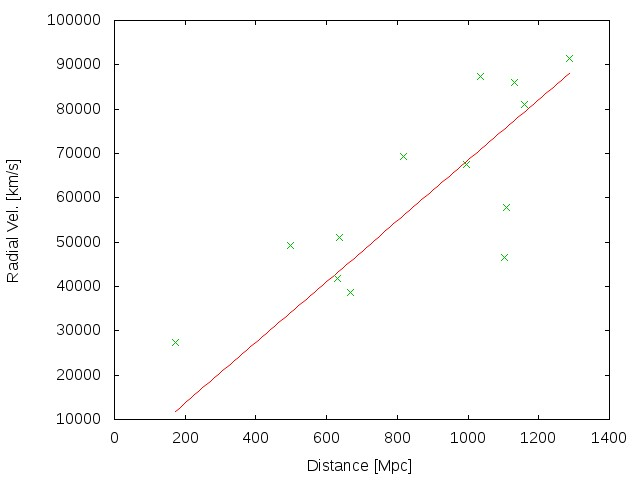
\includegraphics[width=0.7\linewidth]{../pic/HubbleDiagram}
\caption{Hubble diagram: velocity as a function of distance}
\label{fig:HubbleDiagram}
\end{figure}
From figure \ref{fig:bild} we get the Hubble-Constant as:
\begin{equation*}
H_0=\left( 68.8\pm 4.2 \right) kms^{-1}Mpc^{-1}
\end{equation*}
\section*{Exercise C.}

We want to place the galaxies listed below on the colour-magnitude diagram defined by the absolute magnitude $M_u$ in SDSS-$u$ band and the SDSS-($u-r$) colour. These galaxies belong to the Virgo cluster and can be placed to the common distance as defined by $m-M = \SI{31.09}{\mag}$. In order to plot these galaxies, though, we need to correct their photometry for the foreground extinction applied by the dust in the Milky Way along their line of sight. \\

1. Use NED (\url{https://ned.ipac.caltech.edu/forms/byname.html}) to retrieve the galaxy morphology, and the foreground extinction $A_\lambda$ in the SDSS $u$ and $r$ filters as derived from the COBE/DIRBE dust emission maps. Correct the apparent $u$ and $r$ magnitudes for these extinction values. (8 points) \\

The galaxy morphology as well as the foreground extinction corrections $A_\lambda$ have been extracted from NED and are displayed in Table \ref{tab:extinction} together with the given apparent magnitudes in the respective filters. \\

In order to correct the apparent magnitudes in the $u$ and $r$ band with the foreground extinction corrections one does not need to correct the $g$ band values as shown in the following equations with the example values for VCC1226. 

\begin{eqnarray}
 %g &=& \SI{8.53}{\mag} \quad ; \quad A_\lambda \left( g \right) = \SI{0.074}{\mag} \\
 %\Rightarrow g_\text{corr} &=& g - A_\lambda \left( g \right) = \SI{8.456}{\mag} \\
 \left( u-g \right) &=& \SI{1.95}{\mag} \\ 
 \Rightarrow u &=& \left( u-g \right) + g \\
 \Rightarrow u_\text{corr} &=& u - A_\lambda \left( u \right) = \left( u-g \right) + g - A_\lambda \left( u \right) = \SI{10.386}{\mag} \\
\end{eqnarray}

\begin{eqnarray}
 \left( g-r \right) &=& \SI{0.81}{\mag} \\
 \Rightarrow r &=& g - \left( g-r \right) \\
 \Rightarrow r_\text{corr} &=& r - A_\lambda \left( r \right) = g - \left( g-r \right) - A_\lambda \left( r \right) = \SI{7.669}{\mag}
\end{eqnarray}

Similarly, the corrected magnitudes in the $u$ and $r$ band have been computed for all galaxies. To obtain the absulute magnitude in these two bands the value of \SI{31.09}{\mag} is subtracted from the apparent magnitudes as was explained in the task. The corrected apparent and the computed absolute magnitudes as well as the difference between the absolute magnitudes in the $u$ and $r$ band are displayed in Table \ref{tab:magnitude}. \\


% \begin{table}[h!]
% \centering
% \begin{tabular}{cc|ccc|ccc}\toprule
% Galaxy  & morphology & $g$ & $u-g$ & $g-r$ & $A_\lambda \left( g \right)$ & $A_\lambda \left( u \right)$ & $A_\lambda \left( r \right)$ \\
%  & & [\si{\mag}] & [\si{\mag}] & [\si{\mag}] & [\si{\mag}] & [\si{\mag}] & [\si{\mag}] \\ \midrule
% VCC1226 & \verb E2 & 8.53 & 1.95 & 0.81 & 0.074 & 0.094 & 0.051 \\
% VCC0763 & \verb E1 & 9.18 & 1.90 & 0.78 & 0.134 & 0.172 & 0.093 \\
% VCC1231 & \verb E5 & 10.34 & 1.86 & 0.76 & 0.093 & 0.119 & 0.064 \\
% VCC1154 & \verb SA0^+(r) & 10.69 & 1.82 & 0.7 & 0.149 & 0.191 & 0.103 \\
% VCC2000 & \verb E? & 11.65 & 1.81 & 0.75 & 0.113 & 0.145 & 0.078 \\
% VCC0944 & \verb SB0?_edge-on & 11.66 & 1.72 & 0.76 & 0.081 & 0.104 & 0.056 \\
% VCC1619 & \verb SB0^0?_edge-on & 12.11 & 1.82 & 0.71 & 0.131 & 0.169 & 0.091 \\
% VCC1537 & \verb S0^0? & 12.57 & 1.62 & 0.78 & 0.151 & 0.193 & 0.104 \\
% VCC0828 & \verb E & 12.66 & 1.82 & 0.74 & 0.109 & 0.140 & 0.075 \\
% VCC1178 & \verb S? & 13.03 & 1.71 & 0.74 & 0.072 & 0.092 & 0.050 \\
% VCC1857 & \verb Im? & 14.82 & 1.30 & 0.53 & 0.083 & 0.107 & 0.057 \\
% VCC1075 & \verb (no_entry) & 14.81 & 1.39 & 0.70 & 0.089 & 0.114 & 0.062 \\
% VCC1948 & \verb (no_entry) & 15.38 & 1.34 & 0.58 & 0.083 & 0.106 & 0.057 \\
% VCC0230 & \verb (no_entry) 15.50 & 1.44 & 0.64 & & 0.092 & 0.118 & 0.063 \\
% VCC1828 & \verb Scd? & 14.91 & 1.35 & 0.68 & 0.122 & 0.157 & 0.084 \\
% \bottomrule
% \end{tabular}
% \caption{}
% \label{tab:extinction}
% \end{table}

\begin{table}[!ht]
\centering
\begin{tabular}{cc|ccc|cc}\toprule
Galaxy  & morphology & $g$ & $u-g$ & $g-r$ & $A_\lambda \left( u \right)$ & $A_\lambda \left( r \right)$\\
 & & [\si{\mag}] & [\si{\mag}] & [\si{\mag}] & [\si{\mag}] & [\si{\mag}] \\ \midrule
VCC1226 & \verb E2 & 8.53 & 1.95 & 0.81 & 0.094 & 0.051 \\
VCC0763 & \verb E1 & 9.18 & 1.90 & 0.78 & 0.172 & 0.093 \\
VCC1231 & \verb E5 & 10.34 & 1.86 & 0.76 & 0.119 & 0.064 \\
VCC1154 & \verb SA0^+(r) & 10.69 & 1.82 & 0.7 & 0.191 & 0.103 \\
VCC2000 & \verb E? & 11.65 & 1.81 & 0.75 & 0.145 & 0.078 \\
VCC0944 & \verb SB0?_edge-on & 11.66 & 1.72 & 0.76 & 0.104 & 0.056 \\
VCC1619 & \verb SB0^0?_edge-on & 12.11 & 1.82 & 0.71 & 0.169 & 0.091 \\
VCC1537 & \verb S0^0? & 12.57 & 1.62 & 0.78 & 0.193 & 0.104 \\
VCC0828 & \verb E & 12.66 & 1.82 & 0.74 & 0.140 & 0.075 \\
VCC1178 & \verb S? & 13.03 & 1.71 & 0.74 & 0.092 & 0.050 \\
VCC1857 & \verb Im? & 14.82 & 1.30 & 0.53 & 0.107 & 0.057 \\
VCC1075 & \verb (no_entry) & 14.81 & 1.39 & 0.70 & 0.114 & 0.062 \\
VCC1948 & \verb (no_entry) & 15.38 & 1.34 & 0.58 & 0.106 & 0.057 \\
VCC0230 & \verb (no_entry) & 15.50 & 1.44 & 0.64 & 0.118 & 0.063 \\
VCC1828 & \verb Scd? & 14.91 & 1.35 & 0.68 & 0.157 & 0.084 \\
\bottomrule
\end{tabular}
\caption{Uncorrected apparent magnitudes in different bands and foreground extinction coefficients.}
\label{tab:extinction}
\end{table}

\begin{table}[!ht]
\centering
\begin{tabular}{c|cc|cc|c}\toprule
Galaxy & $u_\text{corr}$ & $r_\text{corr}$ & $M_u$ & $M_r$ & $M_u - M_r$ \\
 & [\si{\mag}] & [\si{\mag}] & [\si{\mag}] & [\si{\mag}] & [\si{\mag}] \\ \midrule
VCC1226 & $10.386$ & $7.669$ & $-20.704$ & $-23.421$ & $2.717$ \\
VCC0763 & $10.908$ & $8.307$ & $-20.182$ & $-22.783$ & $2.601$ \\
VCC1231 & $12.081$ & $9.516$ & $-19.009$ & $-21.574$ & $2.565$ \\
VCC1154 & $12.319$ & $9.837$ & $-18.771$ & $-21.253$ & $2.482$ \\
VCC2000 & $13.315$ & $10.822$ & $-17.775$ & $-20.268$ & $2.493$ \\
VCC0944 & $13.276$ & $10.844$ & $-17.814$ & $-20.246$ & $2.432$ \\
VCC1619 & $13.761$ & $11.309$ & $-17.329$ & $-19.781$ & $2.452$ \\
VCC1537 & $13.997$ & $11.686$ & $-17.093$ & $-19.404$ & $2.311$ \\
VCC0828 & $14.340$ & $11.845$ & $-16.750$ & $-19.245$ & $2.495$ \\
VCC1178 & $14.648$ & $12.240$ & $-16.442$ & $-18.850$ & $2.408$ \\
VCC1857 & $16.013$ & $14.233$ & $-15.077$ & $-16.857$ & $1.780$ \\
VCC1075 & $16.086$ & $14.048$ & $-15.004$ & $-17.042$ & $2.038$ \\
VCC1948 & $16.614$ & $14.743$ & $-14.476$ & $-16.347$ & $1.871$ \\
VCC0230 & $16.822$ & $14.797$ & $-14.268$ & $-16.293$ & $2.025$ \\
VCC1828 & $16.103$ & $14.146$ & $-14.987$ & $-16.944$ & $1.957$ \\
\bottomrule
\end{tabular}
\caption{Corrected apparent magnitude and calculated absolute magnitude for the galaxies of the Virgo cluster.}
\label{tab:magnitude}
\end{table}

2. Plot $M_u$ along the x-axis and ($u-r$) along the y-axis, already corrected for foreground extinction, and briefly comment any possible trend visible on this colour-magnitude diagram as a function of galaxy morphology. (3 points) \\

The plot with the computed absolute magnitude in the $u$ band on the x-axis and the difference of the absolute magitudes in the $u$ and $r$ bands on the y-axis can be seen in Figure \ref{fig:cmd_Virgo}. A general trend of brighter galaxies having a larger $(u-r)$ value can be observed. This means that brighter galaxies are correlated with bluer light which may come from larger stars having both increased brightness and an emission spectrum brighter in the blue wavelength region. \\

\begin{figure}[!ht]
\centering
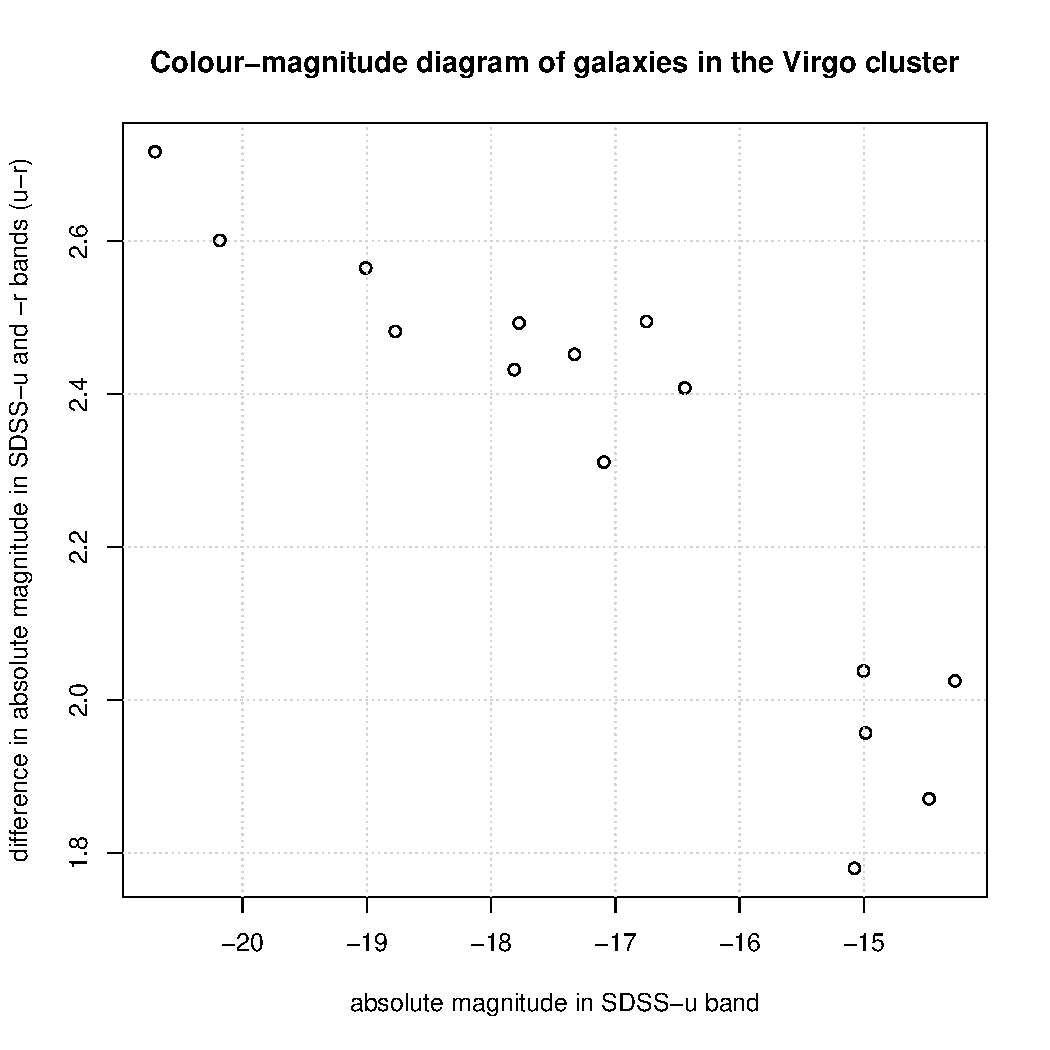
\includegraphics[width=1\linewidth]{pic/cmd_Virgo.pdf}
\caption{Colour-magnitude diagram of galaxies in the Virgo cluster.}
\label{fig:cmd_Virgo}
\end{figure}

\end{document}
